% Provenance (never printed): old premiere S material on the formation of fossil
% fuels (preserved organic matter, burial, oil window, migration, trap, coal).
% Burial history of the invented Merrow Basin from figdata/grade-11/oil_window.py
% (constant geotherm, no compaction). Rifts and passive margins after the USGS
% West-Central Coastal Province fact sheet (2023-3028). Folds are defined in
% g12.02 mountain-building (Sync 0): the anticline is told in prose here, never
% defined. Sedimentary basins compared, diagenesis: Year 1/2.
\chapter{The Geology of Coal, Oil and Gas}\label{ch:g11:fossil-fuel-geology}

A \omterm{def:g11:subduction-zones:slab}{slab} of black shale taken from an old \omterm{def:g11:fossil-fuel-geology:coal}{coal} mine in Pennsylvania carries the
leaves of fern-like plants, flattened and silvery against the dark rock. They
grew in a swamp more than three hundred million years ago, in the
Carboniferous; buried before they could rot, they kept their shape, and the
carbon of the swamp's plants became \omterm{def:g11:fossil-fuel-geology:coal}{coal}. Oil and gas, pumped today from
platforms out at sea, have the same kind of origin: the remains of living
things that escaped decay and were then buried and heated. This chapter
follows that buried carbon from the swamp and the sea floor to the \omterm{def:g11:fossil-fuel-geology:coal}{coal} seam
and the oil field.
% ledger: photo:g11-fossil-plants, ics:base.Carboniferous, ics:base.Permian, earle:coal-formation, earle:organic-preservation

\begin{omfigure}
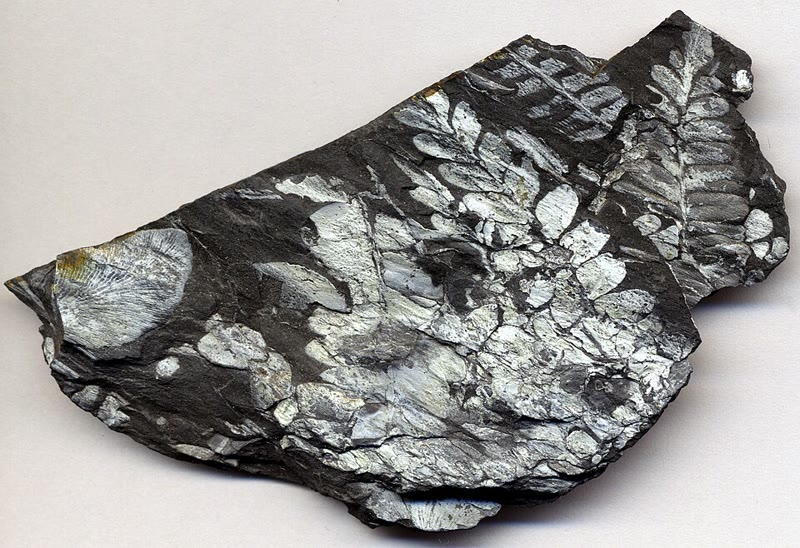
\includegraphics[height=4.4cm]{images/book2/g11-stjohn-fossil-plants.jpg}\hspace{0.03\linewidth}%
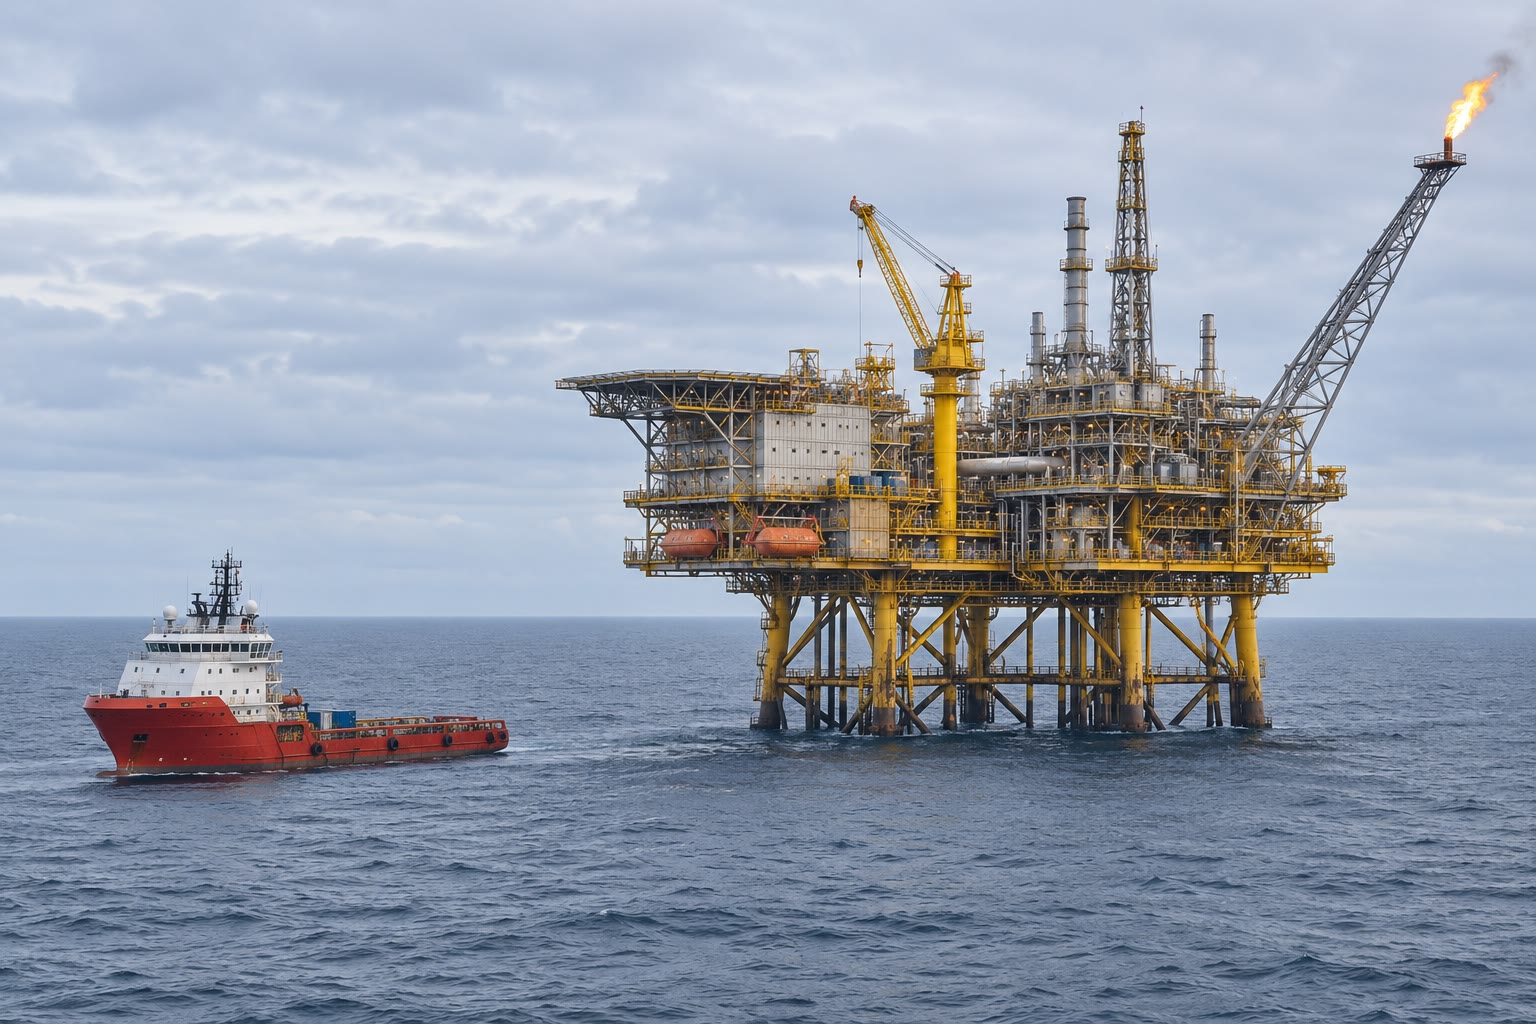
\includegraphics[height=4.4cm]{images/book2/ai/g11-offshore-platform.jpg}

{\small Left: fossil plant leaves in carbon-rich shale from an old \omterm{def:g11:fossil-fuel-geology:coal}{coal}
mine, Pennsylvania, Carboniferous; the \omterm{def:g11:subduction-zones:slab}{slab} is about \qty{10}{cm} across.
Photograph James St.~John (CC~BY~2.0). Right: an oil and gas production
platform at sea (AI illustration).}
\end{omfigure}
% ledger: photo:g11-fossil-plants

\begin{recall}
\omterm{def:g11:fossil-fuel-geology:coal}{Coal}, oil and natural gas are fossil fuels: oil and gas are mixtures of
hydrocarbons, compounds of carbon and hydrogen, and burning a fossil fuel
releases energy and carbon dioxide (the chemistry books). Plants and algae
make organic matter from carbon dioxide and water by photosynthesis (the
biology books). \omterm{def:g11:fossil-fuel-geology:coal}{Coal}, oil and gas come from organic matter buried in
sediments, and they are stored in sedimentary rocks (Book 1, grade 9). A rock
is porous when it holds empty spaces, permeable when water can flow through
it (Book 1, grade 6). Temperature rises with depth along the \omterm{def:g11:lithosphere-asthenosphere:geotherm}{geotherm},
by 25 to \qty{30}{\degreeCelsius} per kilometre in the first kilometres
(\cref{ch:g11:lithosphere-asthenosphere}).
\end{recall}
% ledger: usgs:gradient-29, earle:organic-preservation

\section{Preserving organic matter}

Most organic matter never becomes a fuel. A dead leaf or a dead alga is
eaten by animals and bacteria or reacts with the oxygen of the air: within
weeks or years its carbon has returned to the atmosphere as carbon dioxide.
Organic matter survives only where it is cut off from oxygen --- at the
bottom of a stagnant swamp, or on a sea floor or lake floor whose water holds
no oxygen. Buried there under more sediment, it can be kept for tens or
hundreds of millions of years.
% ledger: earle:organic-preservation

\omterm{def:g11:fossil-fuel-geology:coal}{Coal} comes mostly from land plants that piled up in swamps. Oil and gas come
mostly from the microscopic algae and other plankton of the sea: where the
surface waters are very productive, dead plankton rains onto the sea floor
fast enough for some of it to escape decay, and it is buried in the mud.
% ledger: earle:coal-formation, earle:oil-window

\begin{definition}[Source rock; kerogen]\label{def:g11:fossil-fuel-geology:source-rock}
\emph{Kerogen}\index{kerogen} is the organic matter scattered in a
sedimentary rock, in small particles that do not dissolve in organic
solvents. A \emph{source rock}\index{source rock} is a sedimentary rock rich
in kerogen, in which oil and gas form when it is buried and heated.
\end{definition}
% ledger: peters08:kerogen, earle:migration-traps

Most \omterm{def:g11:fossil-fuel-geology:source-rock}{source rocks} are shales and mudstones, laid down as muds rich in
organic matter. Near the surface their \omterm{def:g11:fossil-fuel-geology:source-rock}{kerogen} stays solid: bacteria living
without oxygen turn some of the organic matter into methane, but most of
that methane escapes back to the surface. Making oil takes heat, and heat takes depth.
% ledger: earle:oil-window, peters08:kerogen

\section{Burial and maturation}

\begin{definition}[Sedimentary basin]\label{def:g11:fossil-fuel-geology:basin}
A \emph{sedimentary basin}\index{sedimentary basin} is a region of the crust
that sinks over millions of years, so that sediments pile up in it, often
several kilometres thick.
\end{definition}
% ledger: usgs23:rift-salt

In a sinking basin, each layer is buried deeper and deeper under the layers
that pile up on top of it. As it goes down, it follows the \omterm{def:g11:lithosphere-asthenosphere:geotherm}{geotherm}: it is
heated. Its \omterm{def:g11:fossil-fuel-geology:source-rock}{kerogen} is slowly cooked, its large molecules broken into the
smaller ones of oil and gas.
% ledger: earle:oil-window

\begin{definition}[Maturation; oil window; gas window]\label{def:g11:fossil-fuel-geology:oil-window}
The \emph{maturation}\index{maturation} of a \omterm{def:g11:fossil-fuel-geology:source-rock}{source rock} is the
transformation of its \omterm{def:g11:fossil-fuel-geology:source-rock}{kerogen} into oil and gas as it is buried and heated.
The \emph{oil window}\index{oil window} is the range of temperature, from
about 60 to \qty{120}{\degreeCelsius}, in which the \omterm{def:g11:fossil-fuel-geology:source-rock}{kerogen} mostly forms oil.
Beyond about \qty{120}{\degreeCelsius}, in the \emph{gas
window}\index{gas window}, it forms mostly methane.
\end{definition}
% ledger: earle:oil-window, magoon00:tps

Because the temperature rises with depth, the \omterm{def:g11:fossil-fuel-geology:oil-window}{oil window} is also a range of
depths. Where the \omterm{def:g11:lithosphere-asthenosphere:geotherm}{geotherm} is a straight line, it is easy to find.

\begin{proposition}[Depth of the oil window]\label{prop:g11:fossil-fuel-geology:window-depth}
Let the temperature be $T_0$ at the surface and rise with depth $z$ at a
constant \omterm{def:g11:lithosphere-asthenosphere:geotherm}{geothermal gradient} $G$: $T = T_0 + G z$. Then the \omterm{def:g11:fossil-fuel-geology:oil-window}{oil window} lies
between the depths
\[
  z_{\text{top}} = \frac{60 - T_0}{G}
  \qquad\text{and}\qquad
  z_{\text{base}} = \frac{120 - T_0}{G},
\]
temperatures in \unit{\degreeCelsius}. Its thickness is $60/G$: the
steeper the \omterm{def:g11:lithosphere-asthenosphere:geotherm}{geotherm}, the shallower and the thinner the window.
\end{proposition}
% ledger: earle:oil-window

\begin{proof}
The top of the window is the depth where $T_0 + G z = 60$, that is
$z = (60 - T_0)/G$; the base is where $T_0 + G z = 120$. The difference is
$(120 - 60)/G = 60/G$.
\end{proof}

With a surface at \qty{20}{\degreeCelsius} and a gradient of
\qty{30}{\degreeCelsius} per kilometre, the \omterm{def:g11:fossil-fuel-geology:oil-window}{oil window} lies between
$40/30 \approx \qty{1.3}{km}$ and $100/30 \approx \qty{3.3}{km}$. In drill
holes across the United States, the gradient averages
\qty{29}{\degreeCelsius} per kilometre, \num{25} in the east and \num{34}
in the west; a \omterm{def:g11:fossil-fuel-geology:source-rock}{source rock} usually has to be buried more than about
\qty{2}{km} before it makes oil. When no measurement of the \omterm{def:g11:fossil-fuel-geology:source-rock}{kerogen} is
available, petroleum geologists have taken a \omterm{def:g11:fossil-fuel-geology:source-rock}{source rock} buried under more
than about \qty{3}{km} of younger rocks as mature.
% values (oil_window.py): z_top_km 1.3333, z_base_km 3.3333
% ledger: usgs:gradient-29, earle:oil-window, magoon00:tps

\begin{omfigure}
\begin{tikzpicture}
\begin{axis}[omrecord, omage, omdepth, name=burial, width=0.54\linewidth, height=5.6cm,
  xmin=0, xmax=170, ymin=0, ymax=4.5, xlabel={age (millions of years ago)},
  ylabel={depth (\unit{km})}, unbounded coords=jump, clip=false,
  xtick={0,20,...,160}, ytick={0,1,...,4}]
\fill[omProp!18] (axis cs:170,1.3333) rectangle (axis cs:0,3.3333);
\fill[omThm!12] (axis cs:170,3.3333) rectangle (axis cs:0,4.5);
\node[font=\scriptsize, anchor=west, text=omProp!80!black] at (axis cs:168,1.75) {oil window};
\node[font=\scriptsize, anchor=west, text=omThm] at (axis cs:168,3.9) {gas window};
\node[font=\scriptsize, anchor=south west, text=black!60, inner sep=1pt] at (axis cs:168,1.3333) {\qty{60}{\degreeCelsius}};
\node[font=\scriptsize, anchor=south west, text=black!60, inner sep=1pt] at (axis cs:168,3.3333) {\qty{120}{\degreeCelsius}};
% computed in figdata/grade-11/oil_window.py (invented basin)
\addplot[black!45, line width=0.6pt] table[x=age, y=z150] {figdata/out/grade-11-oil_window-history.dat};
\addplot[black!45, line width=0.6pt] table[x=age, y=z120] {figdata/out/grade-11-oil_window-history.dat};
\addplot[black!45, line width=0.6pt] table[x=age, y=z95] {figdata/out/grade-11-oil_window-history.dat};
\addplot[black!45, line width=0.6pt] table[x=age, y=z66] {figdata/out/grade-11-oil_window-history.dat};
\addplot[black, line width=1.4pt] table[x=age, y=z165] {figdata/out/grade-11-oil_window-history.dat};
\draw[omDef, dashed, line width=0.8pt] (axis cs:80,0) -- (axis cs:80,4.5);
\node[font=\scriptsize, anchor=west, text=omDef, inner sep=1pt] at (axis cs:78,4.2) {anticline forms};
\fill[omThm] (axis cs:116.97,1.3333) circle (2pt);
\fill[omThm] (axis cs:51.24,3.3333) circle (2pt);
\node[font=\scriptsize, anchor=north east, inner sep=1pt] at (axis cs:100,2.3) {source rock};
\end{axis}
\begin{axis}[omrecord, omdepth, at={(burial.east)}, anchor=west, xshift=1.7cm, width=0.34\linewidth, height=5.6cm,
  xmin=15, xmax=50, ymin=0, ymax=7, xlabel={gradient (\unit{\degreeCelsius/km})},
  ylabel={depth (\unit{km})}]
% computed in figdata/grade-11/oil_window.py (proposition, surface at 20 degC)
\addplot[name path=top, omProp, line width=1pt] table[x=G, y=z_top] {figdata/out/grade-11-oil_window-windows.dat};
\addplot[name path=base, omThm, line width=1pt] table[x=G, y=z_base] {figdata/out/grade-11-oil_window-windows.dat};
\addplot[omProp!18] fill between[of=top and base];
\node[font=\scriptsize] at (axis cs:40,1.75) {oil window};
\node[font=\scriptsize, anchor=south, text=omProp!80!black] at (axis cs:42,0.95) {top};
\node[font=\scriptsize, anchor=north west, text=omThm] at (axis cs:24,4.6) {base};
\end{axis}
\end{tikzpicture}

{\small Left: burial history of the Merrow Basin, an invented basin (computed
model, compaction ignored). Each line follows one layer through time, from
the day it was laid down at the surface; the thick line is the \omterm{def:g11:fossil-fuel-geology:source-rock}{source rock},
laid down 165 million years ago. With the surface at
\qty{20}{\degreeCelsius} and a gradient of \qty{30}{\degreeCelsius} per
kilometre, the \omterm{def:g11:fossil-fuel-geology:oil-window}{oil window} is the band between \num{1.3} and
\qty{3.3}{km}. The dots mark when the \omterm{def:g11:fossil-fuel-geology:source-rock}{source rock} entered it and when it
left it, for the \omterm{def:g11:fossil-fuel-geology:oil-window}{gas window}. Right: depth of the top and the base of the \omterm{def:g11:fossil-fuel-geology:oil-window}{oil
window} against the \omterm{def:g11:lithosphere-asthenosphere:geotherm}{geothermal gradient} (surface at
\qty{20}{\degreeCelsius}).}
\end{omfigure}
% values (oil_window.py): enter_oil_Ma 116.97, leave_oil_Ma 51.24, T_max 140 (20 Ma), T_today 125

A diagram like this one is a \emph{burial-history diagram}: age runs from
left to right towards today, depth downwards. It turns a column of rocks,
dated layer by layer, into a story.

\begin{method}[Reading a burial-history diagram]\label{met:g11:fossil-fuel-geology:burial}
\begin{enumerate}
  \item Find the line of the \omterm{def:g11:fossil-fuel-geology:source-rock}{source rock}: it starts at the surface on the
        day the rock was laid down.
  \item Draw the top and the base of the \omterm{def:g11:fossil-fuel-geology:oil-window}{oil window}, as depths, from the
        \omterm{def:g11:lithosphere-asthenosphere:geotherm}{geotherm} (\cref{prop:g11:fossil-fuel-geology:window-depth}).
  \item Read the age at which the \omterm{def:g11:fossil-fuel-geology:source-rock}{source rock}'s line crosses the top of the
        window: the \omterm{def:g11:fossil-fuel-geology:source-rock}{source rock} begins to make oil. Read the age at which it
        crosses the base: from then on it makes gas.
  \item Compare those ages with the age of the \omterm{def:g11:fossil-fuel-geology:trap}{trap}: only oil and gas
        formed after the \omterm{def:g11:fossil-fuel-geology:trap}{trap} exists can be held in it.
\end{enumerate}
\end{method}
% ledger: magoon00:tps

In the Merrow Basin, the \omterm{def:g11:fossil-fuel-geology:source-rock}{source rock} enters the \omterm{def:g11:fossil-fuel-geology:oil-window}{oil window} about 117
million years ago and leaves it about 51 million years ago; its deepest
burial, \qty{4.0}{km} at \qty{140}{\degreeCelsius}, comes 20 million years
ago, before uplift and erosion raise it again. Today it is still in the \omterm{def:g11:fossil-fuel-geology:oil-window}{gas
window}. The weekend problem computes these ages.
% values (oil_window.py): enter_oil_Ma 116.97, leave_oil_Ma 51.24, z_max_km 4, T_max 140, T_today 125

\section{From source to trap}

Oil and gas are lighter than water, and the pores of buried rocks are full of
water. Once formed, they are pushed out of the \omterm{def:g11:fossil-fuel-geology:source-rock}{source rock} and creep upwards,
through any rock that lets them pass.
% ledger: earle:migration-traps

\begin{definition}[Migration]\label{def:g11:fossil-fuel-geology:migration}
\emph{Migration}\index{migration (of oil and gas)} is the slow movement of
oil and gas out of the \omterm{def:g11:fossil-fuel-geology:source-rock}{source rock} where they formed, upwards through
permeable rocks, driven by their lower density than the water around them.
\end{definition}
% ledger: earle:migration-traps

\begin{definition}[Reservoir rock; seal]\label{def:g11:fossil-fuel-geology:reservoir}
A \emph{reservoir rock}\index{reservoir rock} is a porous and permeable
rock in which oil and gas collect: its pores store them, and their links
let them flow towards a well. A \emph{seal}\index{seal (cap rock)} is an
impermeable rock above the reservoir, through which oil and gas cannot
pass.
\end{definition}
% ledger: earle:migration-traps, magoon00:tps

Sandstones and some limestones make good reservoirs; mudstones, shales and
salt make good \omterm{def:g11:fossil-fuel-geology:reservoir}{seals}. Where nothing stops them, oil and gas reach the
surface, where they seep out and are oxidised: their carbon goes back to the
atmosphere. They gather only where a \omterm{def:g11:fossil-fuel-geology:reservoir}{seal} is shaped so that they cannot
slip past it.
% ledger: earle:migration-traps, magoon00:tps

\begin{definition}[Trap]\label{def:g11:fossil-fuel-geology:trap}
A \emph{trap}\index{trap (oil and gas)} is an arrangement of \omterm{def:g11:fossil-fuel-geology:reservoir}{reservoir rock}
and \omterm{def:g11:fossil-fuel-geology:reservoir}{seal} that holds oil and gas in place, closing the way up on every side.
\end{definition}
% ledger: earle:migration-traps

\begin{omfigure}
\begin{tikzpicture}[font=\footnotesize, scale=0.95,
    declare function={hz(\x,\c)=\c+0.1*\x+0.7*exp(-((\x-10)^2)/2.5);}]
  \colorlet{omOil}{green!45!black}\colorlet{omGas}{red!65}
  \fill[omLithShale!70!white] (0,0) rectangle (14,-6.3);
  % overburden: limestone above a sandstone
  \fill[omLithCongl!70!white] (0,0) -- (14,0) -- plot[domain=14:0, samples=80] (\x,{-2.4+0.06*\x+0.3*exp(-((\x-10)^2)/2.5)}) -- cycle;
  \fill[omLithSand!60!white] plot[domain=0:14, samples=80] (\x,{-2.4+0.06*\x+0.3*exp(-((\x-10)^2)/2.5)}) -- plot[domain=14:0, samples=80] (\x,{hz(\x,-3.7)}) -- cycle;
  % seal (mudstone)
  \fill[omLithShale] plot[domain=0:14, samples=80] (\x,{hz(\x,-3.7)}) -- plot[domain=14:0, samples=80] (\x,{hz(\x,-4.4)}) -- cycle;
  % reservoir sandstone
  \fill[omLithSand] plot[domain=0:14, samples=80] (\x,{hz(\x,-4.4)}) -- plot[domain=14:0, samples=80] (\x,{hz(\x,-5.0)}) -- cycle;
  % oil and gas in the crest of the anticline, above the spill depth
  \begin{scope}
    \clip plot[domain=0:14, samples=80] (\x,{hz(\x,-4.4)}) -- plot[domain=14:0, samples=80] (\x,{hz(\x,-5.0)}) -- cycle;
    \fill[omOil] (8,-2.97) rectangle (13,-2.6);
    \fill[omGas] (8,-2.81) rectangle (13,-2.6);
  \end{scope}
  % source rock (black shale)
  \fill[black!70] plot[domain=0:14, samples=80] (\x,{hz(\x,-5.0)}) -- plot[domain=14:0, samples=80] (\x,{hz(\x,-5.6)}) -- cycle;
  \foreach \c in {-3.7,-4.4,-5.0,-5.6}
    \draw[black!55, line width=0.4pt] plot[domain=0:14, samples=80] (\x,{hz(\x,\c)});
  \draw[black!55, line width=0.4pt] plot[domain=0:14, samples=80] (\x,{-2.4+0.06*\x+0.3*exp(-((\x-10)^2)/2.5)});
  \draw[black!70] (0,0) -- (14,0);
  % 60 degC isotherm
  \draw[omThm, dashed, line width=0.8pt] (0,-4.3) -- (14,-4.3);
  \node[anchor=north east, text=omThm, fill=omLithShale!70!white, inner sep=1pt] at (13.95,-4.35) {\qty{60}{\degreeCelsius}};
  % migration
  \foreach \s in {0,1}
    \draw[->, omDef, line width=1.1pt] (2.7+1.2*\s,{-5.1+0.12*\s}) -- (3.2+1.2*\s,{-4.55+0.12*\s});
  \draw[->, omDef, line width=1.1pt] (4.6,-4.3) .. controls (6.5,-4.1) and (8.3,-3.7) .. (9.45,-3.0);
  % labels
  \node[anchor=west, text=white] at (0.15,-5.25) {source rock};
  \node[anchor=west] at (5.2,-5.75) {mature where hotter than \qty{60}{\degreeCelsius}};
  \node[anchor=west] at (0.15,-4.75) {reservoir rock};
  \node[anchor=west] at (0.15,-3.97) {seal};
  \node[anchor=west] at (0.15,-0.4) {overburden};
  \node[anchor=north, text=omDef, fill=omLithShale, inner sep=1pt] at (6.2,-3.62) {migration};
  \draw[black!60] (10.0,-2.72) -- (11.4,-1.95);
  \node[anchor=south west, fill=omLithSand!60!white, inner sep=1pt] at (11.4,-1.95) {gas};
  \draw[black!60] (10.6,-2.88) -- (12.3,-2.55);
  \node[anchor=west, fill=omLithShale, inner sep=1pt] at (12.3,-2.55) {oil};
  \draw[black!60] (12.0,-3.45) -- (12.8,-3.15);
  \node[anchor=south, fill=omLithShale, inner sep=1pt] at (12.85,-3.15) {water};
  \node[anchor=north] at (10,-1.0) {trap: the arch of an anticline};
\end{tikzpicture}

{\small A \omterm{def:g11:fossil-fuel-geology:petroleum-system}{petroleum system} (a drawing, not to scale). The \omterm{def:g11:fossil-fuel-geology:source-rock}{source rock}, deep
on the left, lies below the \qty{60}{\degreeCelsius} isotherm and makes
oil; oil and gas move out of it into the sandstone above and creep up along
it, under the mudstone \omterm{def:g11:fossil-fuel-geology:reservoir}{seal}, to the arch of an anticline. There they gather
by density: gas at the top, oil beneath, water below. The \omterm{def:g11:fossil-fuel-geology:petroleum-system}{overburden} rocks
on top bury the \omterm{def:g11:fossil-fuel-geology:source-rock}{source rock} deep enough to mature it.}
\end{omfigure}
% ledger: earle:migration-traps, magoon00:tps, earle:oil-window

In a \omterm{def:g11:fossil-fuel-geology:trap}{trap}, the fluids sort themselves by density: gas on top, oil beneath,
water at the bottom. The simplest \omterm{def:g11:fossil-fuel-geology:trap}{trap} is an anticline, an arch in
the layers (folds are the subject of \cref{ch:g12:mountain-building}). Faults,
salt domes and changes in the rocks themselves also make \omterm{def:g11:fossil-fuel-geology:trap}{traps}.
% ledger: earle:migration-traps

\begin{omfigure}
\begin{tikzpicture}[font=\footnotesize, scale=0.78]
  \colorlet{omOil}{green!45!black}\colorlet{omGas}{red!65}
  % (a) anticline
  \begin{scope}
    \fill[omLithShale] (0,0) rectangle (4,3);
    \fill[omLithSand] plot[domain=0:4, samples=50] (\x,{1.0+1.0*exp(-((\x-2)^2)/1.2)}) -- plot[domain=4:0, samples=50] (\x,{1.5+1.0*exp(-((\x-2)^2)/1.2)}) -- cycle;
    \begin{scope}
      \clip plot[domain=0:4, samples=50] (\x,{1.0+1.0*exp(-((\x-2)^2)/1.2)}) -- plot[domain=4:0, samples=50] (\x,{1.5+1.0*exp(-((\x-2)^2)/1.2)}) -- cycle;
      \fill[omOil] (0,1.75) rectangle (4,3); \fill[omGas] (0,2.25) rectangle (4,3);
    \end{scope}
    \draw[black!50] (0,0) rectangle (4,3);
    \node[anchor=north, text height=1.6ex, text depth=0.3ex] at (2,-0.05) {(a) anticline};
  \end{scope}
  % (b) fault
  \begin{scope}[xshift=4.6cm]
    \fill[omLithShale] (0,0) rectangle (4,3);
    \begin{scope}
      \clip (0,0) -- (2.9,0) -- (2.3,3) -- (0,3) -- cycle;
      \fill[omLithSand] (0,0.6) -- (4,1.8) -- (4,2.3) -- (0,1.1) -- cycle;
      \clip (0,0.6) -- (4,1.8) -- (4,2.3) -- (0,1.1) -- cycle;
      \fill[omOil] (0,1.45) rectangle (4,3); \fill[omGas] (0,1.75) rectangle (4,3);
    \end{scope}
    \begin{scope}
      \clip (2.9,0) -- (4,0) -- (4,3) -- (2.3,3) -- cycle;
      \fill[omLithSand] (0,-0.6) -- (4,0.6) -- (4,1.1) -- (0,-0.1) -- cycle;
    \end{scope}
    \draw[black, line width=1pt] (2.9,0) -- (2.3,3);
    \draw[black!50] (0,0) rectangle (4,3);
    \node[anchor=north, text height=1.6ex, text depth=0.3ex] at (2,-0.05) {(b) fault};
  \end{scope}
  % (c) salt dome
  \begin{scope}[xshift=9.2cm]
    \fill[omLithShale] (0,0) rectangle (4,3);
    \fill[omLithSand] (0,0.9) -- (1.0,1.2) -- (1.4,1.9) -- (1.4,2.4) -- (1.0,1.7) -- (0,1.4) -- cycle;
    \fill[omLithSand] (4,0.9) -- (3.0,1.2) -- (2.6,1.9) -- (2.6,2.4) -- (3.0,1.7) -- (4,1.4) -- cycle;
    \begin{scope}
      \clip (0,0.9) -- (1.0,1.2) -- (1.4,1.9) -- (1.4,2.4) -- (1.0,1.7) -- (0,1.4) -- cycle;
      \fill[omOil] (0,1.65) rectangle (1.4,3); \fill[omGas] (0,2.05) rectangle (1.4,3);
    \end{scope}
    \begin{scope}
      \clip (4,0.9) -- (3.0,1.2) -- (2.6,1.9) -- (2.6,2.4) -- (3.0,1.7) -- (4,1.4) -- cycle;
      \fill[omOil] (2.6,1.65) rectangle (4,3); \fill[omGas] (2.6,2.05) rectangle (4,3);
    \end{scope}
    \fill[omLithEvap, draw=black!60] (1.4,0) -- (1.4,2.4) .. controls (1.4,2.85) and (2.6,2.85) .. (2.6,2.4) -- (2.6,0) -- cycle;
    \node at (2,1.0) {salt};
    \draw[black!50] (0,0) rectangle (4,3);
    \node[anchor=north, text height=1.6ex, text depth=0.3ex] at (2,-0.05) {(c) salt dome};
  \end{scope}
  % (d) stratigraphic
  \begin{scope}[xshift=13.8cm]
    \fill[omLithShale] (0,0) rectangle (4,3);
    \fill[omLithSand] (0,0.6) -- (3.5,1.95) -- (0,1.3) -- cycle;
    \begin{scope}
      \clip (0,0.6) -- (3.5,1.95) -- (0,1.3) -- cycle;
      \fill[omOil] (0,1.45) rectangle (4,3); \fill[omGas] (0,1.7) rectangle (4,3);
    \end{scope}
    \draw[black!50] (0,0) rectangle (4,3);
    \node[anchor=north, text height=1.6ex, text depth=0.3ex] at (2,-0.05) {(d) pinch-out};
  \end{scope}
\end{tikzpicture}

{\small Four kinds of \omterm{def:g11:fossil-fuel-geology:trap}{trap} (drawings, not to scale): reservoir sandstone in
yellow, sealing mudstone in grey-green, oil in green, gas in red. (a) The
arch of an anticline. (b) A tilted reservoir cut by a fault, against a
mudstone on the other side. (c) Layers bent up against a rising salt dome.
(d) A sandstone that thins out up-slope within mudstone, a \omterm{def:g11:fossil-fuel-geology:trap}{trap} made by a
change in the rocks themselves.}
\end{omfigure}
% ledger: earle:migration-traps

\begin{example}[A trap in an anticline]\label{ex:g11:fossil-fuel-geology:anticline}
A seismic survey maps the top of a sandstone sealed by mudstone. It forms an
arch whose crest lies \qty{1800}{m} below the surface. Around the crest, the
deepest contour line that still closes all the way round lies at
\qty{2050}{m}; below it, the sandstone opens to the side. A well at the crest
finds gas down to \qty{1880}{m}. How tall a column of oil and gas can the
\omterm{def:g11:fossil-fuel-geology:trap}{trap} hold, and how thick is the oil?

\emph{Solution.} Oil and gas fill the arch from the crest downwards; any
that sinks below the last closed contour spills out to the side, at the
\emph{spill point}, and migrates on. The column is at most
$2050 - 1800 = \qty{250}{m}$ tall. If the \omterm{def:g11:fossil-fuel-geology:trap}{trap} is full, gas fills the top
$1880 - 1800 = \qty{80}{m}$ and oil the next $2050 - 1880 = \qty{170}{m}$,
with water below.
\end{example}
% invented numbers; ledger: earle:migration-traps

Each of the pieces --- a \omterm{def:g11:fossil-fuel-geology:source-rock}{source rock}, a reservoir, a \omterm{def:g11:fossil-fuel-geology:reservoir}{seal}, the rocks on top
that bury the \omterm{def:g11:fossil-fuel-geology:source-rock}{source rock}, a \omterm{def:g11:fossil-fuel-geology:trap}{trap} --- is necessary, and they must come in the
right order.

\begin{definition}[Petroleum system]\label{def:g11:fossil-fuel-geology:petroleum-system}
A \emph{petroleum system}\index{petroleum system} is a body of mature \omterm{def:g11:fossil-fuel-geology:source-rock}{source
rock} together with all the oil and gas that came from it, and the elements
and processes they need: the \omterm{def:g11:fossil-fuel-geology:source-rock}{source rock}, the \omterm{def:g11:fossil-fuel-geology:reservoir}{reservoir rock}, the \omterm{def:g11:fossil-fuel-geology:reservoir}{seal} and
the \emph{overburden}\index{overburden} (the rocks above, which bury the
\omterm{def:g11:fossil-fuel-geology:source-rock}{source rock}), and the formation of \omterm{def:g11:fossil-fuel-geology:trap}{traps}, the generation, migration and
accumulation of oil and gas.
\end{definition}
% ledger: magoon00:tps

The order matters most. A \omterm{def:g11:fossil-fuel-geology:trap}{trap} that forms after the oil has gone by catches
nothing: the burial-history diagram dates the generation of oil, the history
of the folds and faults dates the \omterm{def:g11:fossil-fuel-geology:trap}{trap}, and the \omterm{def:g11:fossil-fuel-geology:petroleum-system}{petroleum system} works only
if the \omterm{def:g11:fossil-fuel-geology:trap}{trap} came first. Petroleum geologists also call the time that best
shows generation, migration and accumulation together the \emph{critical
moment}.
% ledger: magoon00:tps

\section{Where oil and gas gather}

Where does a \omterm{def:g11:fossil-fuel-geology:petroleum-system}{petroleum system} come together? It needs a basin that sinks for
a long time, waters poor in oxygen to keep organic matter, and \omterm{def:g11:fossil-fuel-geology:reservoir}{seals}. Rifts
and the continental margins they grow into have all three.
% ledger: usgs23:rift-salt

When a continent begins to split, as Africa does today along the East
African Rift (Book 1, grade 7), its crust stretches and breaks into blocks
along \omterm{def:g11:ocean-ridges:normal-fault}{normal faults} (\cref{ch:g11:ocean-ridges}). Some blocks drop, others
tilt, and the troughs between them fill with sediments, often several
kilometres thick, and with lakes, whose muds rich in organic matter can
become \omterm{def:g11:fossil-fuel-geology:source-rock}{source rocks}. When
stretching stops, the thinned crust cools and keeps sinking slowly, so that
the basin goes on filling. If the sea then floods into a basin only
partly connected to the ocean and evaporates, it leaves thick layers of
salt. Once the rift has opened into an ocean, its edges become passive
margins: continental edges inside a plate, far from any plate boundary, which
go on sinking and receiving sediment from the land.
% ledger: usgs23:rift-salt, usgs:pangaea-breakup

\begin{omfigure}
\begin{tikzpicture}[font=\footnotesize, x=1cm, y=0.8cm]
  \fill[omLithShale] (0,0.25) -- (1.5,0) -- (7,-0.4) -- (10,-2.2) -- (14,-2.6) -- (14,-8.0) -- (0,-8.0) -- cycle;
  % sea and land
  \fill[omSea] (1.5,0) -- (14,0) -- (14,-2.6) -- (10,-2.2) -- (7,-0.4) -- cycle;
  \draw[omRiver!60, line width=0.6pt] (1.5,0) -- (14,0);
  % marine sediments above the salt
  \fill[omLithShale] (0,0.25) -- (1.5,0) -- (7,-0.4) -- (10,-2.2) -- (14,-2.6) -- (14,-4.95) -- (11.2,-4.5) -- (11.2,-3.74) -- (0,-2.4) -- cycle;
  \fill[omLithSand] (0,-0.9) -- (6,-1.45) -- (10,-2.75) -- (14,-3.3) -- (14,-3.6) -- (10,-3.05) -- (6,-1.75) -- (0,-1.2) -- cycle;
  % salt layer and a salt dome
  \fill[omLithEvap, draw=black!50] (1.2,-2.25) -- (11.2,-3.74) -- (11.2,-4.14) -- (1.2,-2.65) -- cycle;
  \fill[omLithEvap, draw=black!50] (7.0,-3.0) .. controls (7.3,-2.6) and (7.25,-1.9) .. (7.2,-1.6)
     .. controls (7.4,-1.2) and (8.2,-1.2) .. (8.4,-1.6)
     .. controls (8.35,-2.1) and (8.3,-2.7) .. (8.7,-3.25) -- cycle;
  % continental crust with tilted blocks
  \fill[omLithGranite] (0,-2.75) -- (2.5,-3.0) -- (4.85,-4.6) -- (5.0,-3.4) -- (7.35,-5.0) -- (7.5,-3.75) -- (9.85,-5.3) -- (10.0,-4.1) -- (11.2,-5.0) -- (11.2,-6.0) -- (0,-7.6) -- cycle;
  % rift fill: lake shales (source rocks) in the half-grabens
  \fill[black!65] (2.5,-3.0) -- (4.85,-4.6) -- (5.0,-3.4) -- (4.0,-3.25) -- cycle;
  \fill[black!65] (5.0,-3.4) -- (7.35,-5.0) -- (7.5,-3.75) -- (6.5,-3.6) -- cycle;
  \fill[black!65] (7.5,-3.75) -- (9.85,-5.3) -- (10.0,-4.1) -- (9.0,-3.95) -- cycle;
  \fill[black!65] (2.5,-3.0) -- (4.0,-3.25) -- (5.0,-3.4) -- (6.5,-3.6) -- (7.5,-3.75) -- (9.0,-3.95) -- (10.0,-4.1) -- (11.2,-4.3) -- (11.2,-4.14) -- (1.2,-2.65) -- (1.2,-2.87) -- cycle;
  \draw[black!70, line width=0.8pt] (4.85,-4.6) -- (5.0,-3.4) (7.35,-5.0) -- (7.5,-3.75) (9.85,-5.3) -- (10.0,-4.1);
  % oceanic crust and mantle
  \fill[omLithBasalt] (11.2,-4.5) -- (14,-4.95) -- (14,-6.0) -- (11.2,-6.0) -- cycle;
  \fill[omLithPeridotite] (0,-7.6) -- (11.2,-6.0) -- (14,-6.0) -- (14,-8.0) -- (0,-8.0) -- cycle;
  % oil beside the salt dome
  \fill[green!45!black] (6.85,-1.5) -- (7.22,-1.65) -- (7.22,-1.95) -- (6.85,-1.75) -- cycle;
  \draw[black!60] (0,-8.0) rectangle (14,1.0);
  % labels
  \node[anchor=west] at (11.5,-1.2) {sea};
  \node[anchor=south west] at (0.1,0.3) {land};
  \node[anchor=west, fill=omLithShale, inner sep=1pt] at (2.2,-0.45) {marine sediments};
  \node[anchor=west, fill=omLithEvap, inner sep=1pt] at (9.0,-1.25) {salt dome};
  \draw[black!60] (8.4,-1.4) -- (9.0,-1.25);
  \node[anchor=east, fill=omLithShale, inner sep=1pt] at (6.6,-2.1) {oil};
  \draw[black!60] (6.6,-2.1) -- (6.95,-1.75);
  \node[anchor=west, fill=omLithShale, inner sep=1pt] at (11.4,-3.35) {salt (seal)};
  \draw[black!60] (10.8,-3.7) -- (11.4,-3.35);
  \node[anchor=west, align=left] at (0.3,-4.7) {lake shales\\(source rocks)};
  \draw[black!60] (2.75,-4.45) -- (4.4,-3.8);
  \node[anchor=north, align=center] at (4.0,-5.6) {stretched continental crust:\\tilted blocks and normal faults};
  \node[anchor=north, align=center] at (12.6,-5.05) {oceanic crust};
  \node[anchor=north] at (6,-7.35) {mantle};
\end{tikzpicture}

{\small A passive margin built on an old rift (a drawing, not to scale, depths
exaggerated). In the rift, tilted blocks of continental crust bounded by
\omterm{def:g11:ocean-ridges:normal-fault}{normal faults} hold lake shales, the \omterm{def:g11:fossil-fuel-geology:source-rock}{source rocks}. A layer of salt, laid down
when the young sea evaporated, \omterm{def:g11:fossil-fuel-geology:reservoir}{seals} them; above it, marine sediments pile
up as the margin sinks. Salt, lighter than the sediments around it, rises
in domes that bend the layers into \omterm{def:g11:fossil-fuel-geology:trap}{traps}.}
\end{omfigure}
% ledger: usgs23:rift-salt, earle:migration-traps

The margins of the South Atlantic were built this way. Africa and South
America began to separate in the Late Triassic or Early Jurassic. Off
western Central Africa, the rift troughs filled with several kilometres of
sediments, among them lake shales up to \qty{600}{m} thick holding up to
\qty{20}{\percent} of organic carbon by mass. In the Early Cretaceous the sea
began to flood in, again and again, and evaporated, leaving more than a
kilometre of salt; where the salt has stayed in place, it \omterm{def:g11:fossil-fuel-geology:reservoir}{seals} the oil and
gas of the rocks below. In the Gulf of Mexico, salt that is lighter than the
sediments around it has risen in domes, and the layers bent against them
are \omterm{def:g11:fossil-fuel-geology:trap}{traps}.
% ledger: usgs23:rift-salt, earle:migration-traps

\section{Coal}

\omterm{def:g11:fossil-fuel-geology:coal}{Coal} forms on land, mostly in swamps beside rivers and deltas, in humid
climates from tropical to temperate, where plants grow fast and their remains
fall into stagnant water poor in oxygen. Over centuries to millennia they pile
up as peat. When a river changes course, or the sea rises, sand and mud bury
the peat; buried deeper, it is squeezed and heated.
% ledger: earle:coal-formation

\begin{definition}[Coal; coalification; rank]\label{def:g11:fossil-fuel-geology:coal}
\emph{Coal}\index{coal} is a sedimentary rock made mostly of the remains of
land plants, rich in carbon. \emph{Coalification}\index{coalification} is the
transformation of peat into coal and of coal into richer coal, by burial and
heating. The \emph{rank}\index{rank (of coal)} of a coal is how far
coalification has gone: from lignite through subbituminous and bituminous
coal to anthracite, the carbon content rises.
\end{definition}
% ledger: earle:coal-formation, eia:coal-carbon

Lignite forms at depths from a few hundred metres to about \qty{1.5}{km},
up to about \qty{50}{\degreeCelsius}; bituminous \omterm{def:g11:fossil-fuel-geology:coal}{coal} between 1 and
\qty{5}{km}, up to about \qty{150}{\degreeCelsius}; anthracite beyond
\qty{5}{km} and \qty{150}{\degreeCelsius}. As the \omterm{def:g11:fossil-fuel-geology:coal}{rank} rises, carbon makes
up more and more of the \omterm{def:g11:fossil-fuel-geology:coal}{coal}: about
25 to \qty{35}{\percent} in lignite, up to 86 to \qty{97}{\percent} in
anthracite. Methane formed on the way stays in the pores of the \omterm{def:g11:fossil-fuel-geology:coal}{coal}, which
is why a \omterm{def:g11:fossil-fuel-geology:coal}{coal} mine can hold explosive gas. Forming a \omterm{def:g11:fossil-fuel-geology:coal}{coal} seam takes millions
of years.
% ledger: earle:coal-formation, eia:coal-carbon

\begin{omfigure}
\begin{tikzpicture}
\begin{axis}[omrecord, xbar, name=rank, width=0.5\linewidth, height=4.6cm, xmin=0, xmax=100,
  ymin=0.4, ymax=4.6, ytick={1,2,3,4},
  yticklabels={lignite, subbituminous, bituminous, anthracite},
  xlabel={carbon content (\unit{\percent})}, ymajorgrids=false]
% ledger: eia:coal-carbon
\fill[omProp!60!black!35] (axis cs:25,0.7) rectangle (axis cs:35,1.3);
\fill[omProp!70!black!55] (axis cs:35,1.7) rectangle (axis cs:45,2.3);
\fill[black!60] (axis cs:45,2.7) rectangle (axis cs:86,3.3);
\fill[black!85] (axis cs:86,3.7) rectangle (axis cs:97,4.3);
\node[font=\scriptsize, anchor=west] at (axis cs:36,1) {25--35};
\node[font=\scriptsize, anchor=west] at (axis cs:46,2) {35--45};
\node[font=\scriptsize, anchor=east, text=white] at (axis cs:85,3) {45--86};
\node[font=\scriptsize, anchor=east] at (axis cs:85,4) {86--97};
\end{axis}
\node[anchor=west] at ([xshift=0.6cm]rank.east) {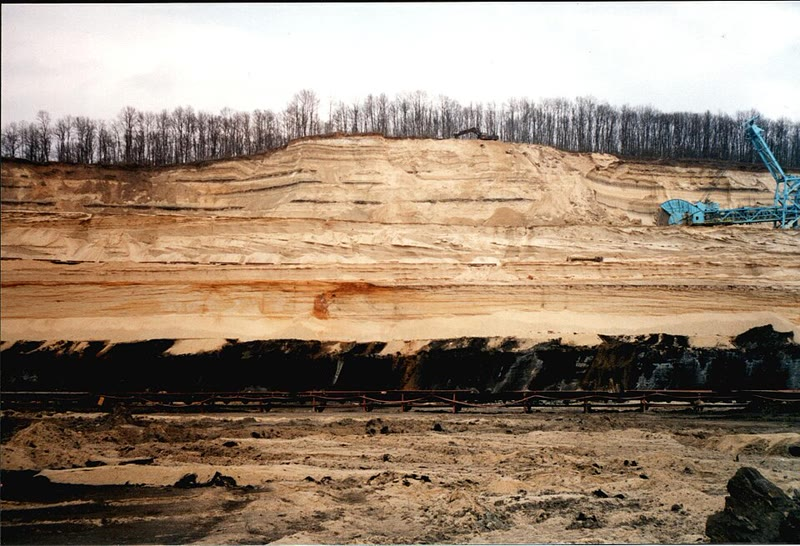
\includegraphics[height=4.0cm]{images/book2/g11-usgs-lignite-bed.jpg}};
\end{tikzpicture}

\medskip
\makebox[0.32\linewidth]{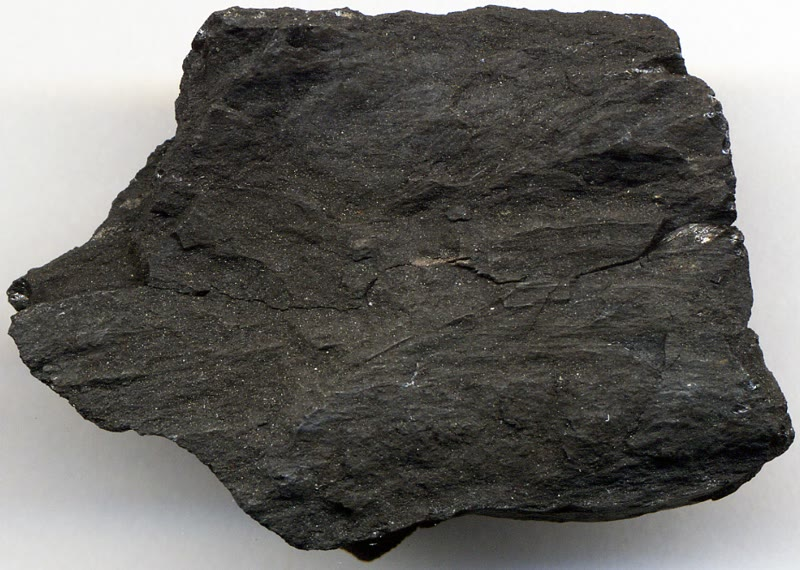
\includegraphics[height=3.2cm]{images/book2/g11-stjohn-lignite.jpg}}\hfill
\makebox[0.32\linewidth]{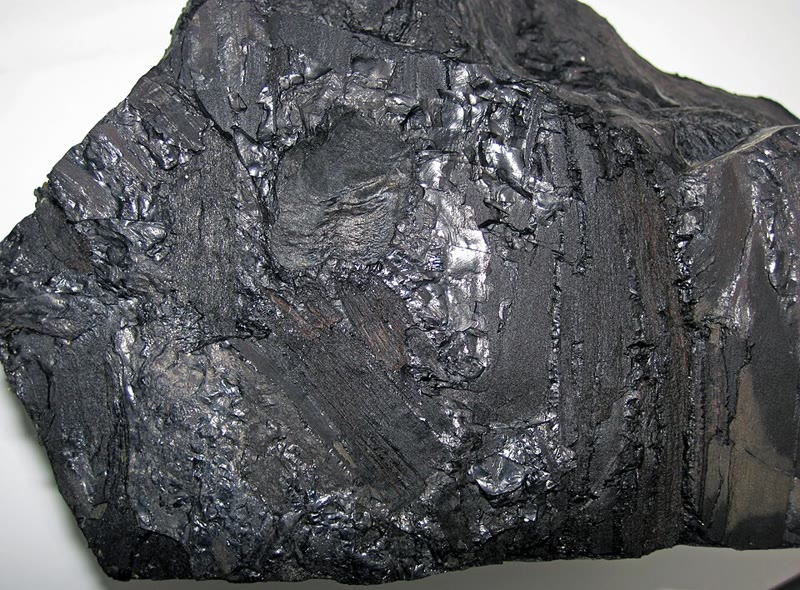
\includegraphics[height=3.2cm]{images/book2/g11-stjohn-bituminous.jpg}}\hfill
\makebox[0.32\linewidth]{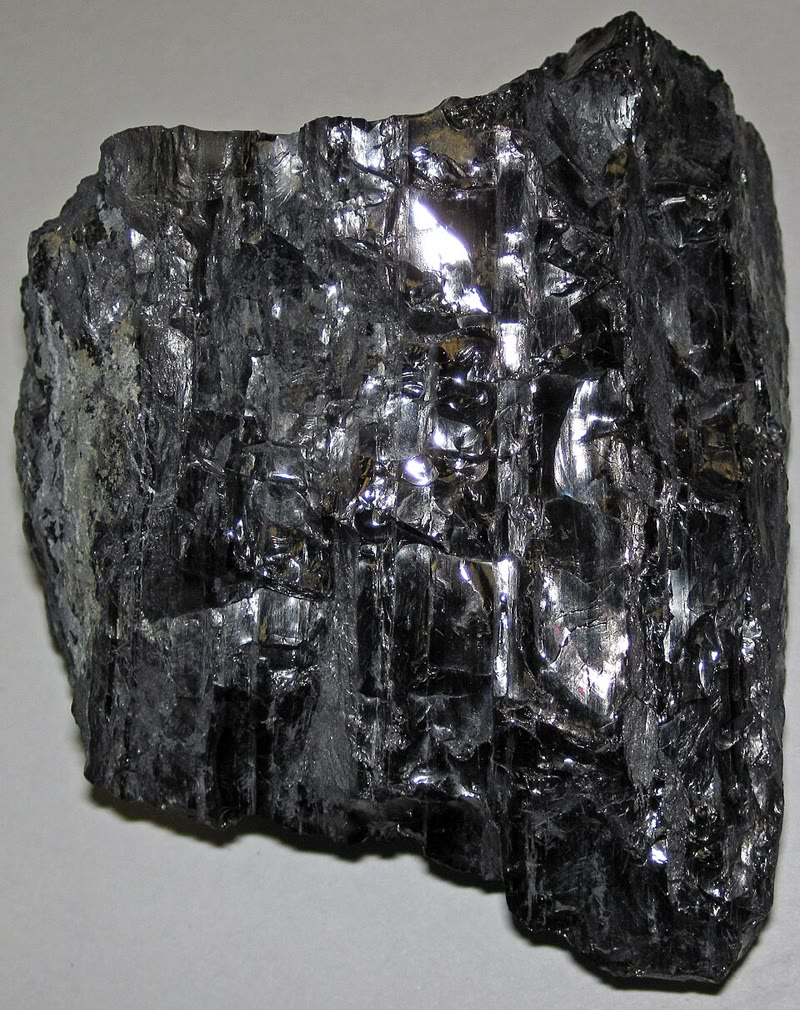
\includegraphics[height=3.2cm]{images/book2/g11-stjohn-anthracite.jpg}}

{\small Top left: carbon content of the \omterm{def:g11:fossil-fuel-geology:coal}{ranks} of \omterm{def:g11:fossil-fuel-geology:coal}{coal}. Data: U.S. Energy
Information Administration. Top right: a bed of lignite, the black band
under pale sands, exposed in a mine in Romania; photograph U.S. Geological
Survey (public domain). Bottom, from left: lignite, about \qty{4.5}{cm}
across, brown-black and dull; bituminous \omterm{def:g11:fossil-fuel-geology:coal}{coal}, with flattened plant
fragments; anthracite, black and glassy. Photographs James St.~John
(CC~BY~2.0).}
\end{omfigure}
% ledger: eia:coal-carbon, photo:g11-lignite-bed, photo:g11-coal-ranks

Peat loses most of its volume on the way. In a \omterm{def:g11:fossil-fuel-geology:coal}{coal} bed of central Utah,
comparing the peat cut away by an ancient river channel with the \omterm{def:g11:fossil-fuel-geology:coal}{coal} missing
beside it gives a ratio of thicknesses of about $11{:}1$: every metre of that
bituminous \omterm{def:g11:fossil-fuel-geology:coal}{coal} was once some eleven metres of peat.
% ledger: ryer80:peat-coal

\section{Exercises}

\begin{exercise}[$\star$]\label{exo:g11:fossil-fuel-geology:1}
Put in order the steps that lead from plankton to oil in a \omterm{def:g11:fossil-fuel-geology:trap}{trap}: migration;
\omterm{def:g11:fossil-fuel-geology:oil-window}{maturation} in the \omterm{def:g11:fossil-fuel-geology:oil-window}{oil window}; burial under younger sediments; dead plankton
settles on a sea floor poor in oxygen; oil gathers under a \omterm{def:g11:fossil-fuel-geology:reservoir}{seal}; the organic
matter becomes \omterm{def:g11:fossil-fuel-geology:source-rock}{kerogen} in a mud.
\end{exercise}

\begin{exercise}[$\star$]\label{exo:g11:fossil-fuel-geology:2}
For each rock, say whether it is more likely a \omterm{def:g11:fossil-fuel-geology:source-rock}{source rock}, a \omterm{def:g11:fossil-fuel-geology:reservoir}{reservoir rock}
or a \omterm{def:g11:fossil-fuel-geology:reservoir}{seal}: (1) a dark shale rich in organic matter; (2) a well-sorted
sandstone with connected pores; (3) a layer of salt; (4) a mudstone with no
organic matter; (5) a limestone full of open cavities.
\end{exercise}

\begin{exercise}[$\star$]\label{exo:g11:fossil-fuel-geology:3}
In a basin, the surface is at \qty{10}{\degreeCelsius} and the \omterm{def:g11:lithosphere-asthenosphere:geotherm}{geothermal
gradient} is \qty{25}{\degreeCelsius/km}. Between which depths does the \omterm{def:g11:fossil-fuel-geology:oil-window}{oil
window} lie? How thick is it?
\end{exercise}

\begin{exercise}[$\star$]\label{exo:g11:fossil-fuel-geology:4}
(1) Put lignite, anthracite, bituminous \omterm{def:g11:fossil-fuel-geology:coal}{coal} and peat in order of rising
\omterm{def:g11:fossil-fuel-geology:coal}{rank}. (2) Which has the highest carbon content? (3) Which formed at the
greatest depth and temperature?
\end{exercise}

\begin{exercise}[$\star$]\label{exo:g11:fossil-fuel-geology:5}
(1) In a \omterm{def:g11:fossil-fuel-geology:trap}{trap}, why does gas lie above oil, and oil above water? (2) Why
must the rock above a reservoir be impermeable? Name two rocks that make
good \omterm{def:g11:fossil-fuel-geology:reservoir}{seals}.
\end{exercise}

\begin{exercise}[$\star\star$]\label{exo:g11:fossil-fuel-geology:6}
Two basins have the same surface temperature, \qty{15}{\degreeCelsius}.
Basin A has a gradient of \qty{20}{\degreeCelsius/km}, basin B of
\qty{40}{\degreeCelsius/km}. (1) Compute the depths of the top and the base
of the \omterm{def:g11:fossil-fuel-geology:oil-window}{oil window} in each. (2) A \omterm{def:g11:fossil-fuel-geology:source-rock}{source rock} lies \qty{2}{km} deep in both
basins. What does it make in each? (3) In which basin must a well go deeper
to find oil formed in place?
\end{exercise}

\begin{exercise}[$\star\star$]\label{exo:g11:fossil-fuel-geology:7}
Take the ratio of $11{:}1$ measured in central Utah between the thickness of a
peat and that of the \omterm{def:g11:fossil-fuel-geology:coal}{coal} it became. (1) What thickness of peat made a \omterm{def:g11:fossil-fuel-geology:coal}{coal}
seam \qty{3}{m} thick? (2) Suppose the peat piled up at \qty{1}{mm} a year.
How long did it take to accumulate? (3) Why must the swamp have been sinking
all that time?
\end{exercise}

\begin{exercise}[$\star\star$]\label{exo:g11:fossil-fuel-geology:8}
Use the burial-history diagram of the Merrow Basin (surface
\qty{20}{\degreeCelsius}, gradient \qty{30}{\degreeCelsius/km}). The \omterm{def:g11:fossil-fuel-geology:source-rock}{source
rock} was \qty{1.2}{km} deep 120 million years ago, \qty{2.3}{km} deep 95
million years ago and \qty{4.0}{km} deep 20 million years ago. (1) Compute
its temperature at each date. (2) At each date, was it immature, in the \omterm{def:g11:fossil-fuel-geology:oil-window}{oil
window} or in the \omterm{def:g11:fossil-fuel-geology:oil-window}{gas window}?
\end{exercise}

\begin{exercise}[$\star\star$]\label{exo:g11:fossil-fuel-geology:9}
The top of a reservoir sandstone forms an arch whose crest is \qty{2400}{m}
deep; its deepest closed contour is at \qty{2580}{m}. A well at the crest
finds gas to \qty{2450}{m}, then oil. (1) What is the greatest height of the
column the \omterm{def:g11:fossil-fuel-geology:trap}{trap} can hold? (2) If the \omterm{def:g11:fossil-fuel-geology:trap}{trap} is full, how thick is the oil?
(3) The oil and gas that keep arriving after the \omterm{def:g11:fossil-fuel-geology:trap}{trap} is full: where do they
go?
\end{exercise}

\begin{exercise}[$\star\star$]\label{exo:g11:fossil-fuel-geology:10}
When no measurement of the \omterm{def:g11:fossil-fuel-geology:source-rock}{kerogen} is available, petroleum geologists have
taken a \omterm{def:g11:fossil-fuel-geology:source-rock}{source rock} buried under more than \qty{3}{km} of rocks as mature.
With a surface at \qty{20}{\degreeCelsius}: (1) Which gradient puts
\qty{3}{km} at the top of the \omterm{def:g11:fossil-fuel-geology:oil-window}{oil window}? at its base? (2) With the
gradients of 25 to \qty{34}{\degreeCelsius/km} measured in drill holes,
where does \qty{3}{km} fall? Is the rule reasonable?
\end{exercise}

\begin{exercise}[$\star\star$]\label{exo:g11:fossil-fuel-geology:11}
Three \omterm{def:g11:fossil-fuel-geology:coal}{coal} samples hold \qty{30}{\percent}, \qty{70}{\percent} and
\qty{92}{\percent} of carbon. (1) Give the \omterm{def:g11:fossil-fuel-geology:coal}{rank} of each. (2) Using the
depths and temperatures given in the course, which was buried deepest?
(3) The lignite has a dull, brown-black look; how does the anthracite look?
\end{exercise}

\begin{exercise}[$\star\star\star$]\label{exo:g11:fossil-fuel-geology:12}
Between 120 and 95 million years ago, \qty{1100}{m} of mud piled up in the
Merrow Basin. (1) Compute the rate of burial in metres per million years.
(2) With a gradient of \qty{30}{\degreeCelsius/km}, by how many degrees did
the \omterm{def:g11:fossil-fuel-geology:source-rock}{source rock} warm per million years? (3) Had this rate gone on, how long
would the \omterm{def:g11:fossil-fuel-geology:source-rock}{source rock} have taken to cross the whole \omterm{def:g11:fossil-fuel-geology:oil-window}{oil window}? (4) The
model gives about 66 million years. Why longer?
\end{exercise}

\begin{exercise}[$\star\star\star$]\label{exo:g11:fossil-fuel-geology:13}
In the Merrow Basin, the \omterm{def:g11:fossil-fuel-geology:source-rock}{source rock} was in the \omterm{def:g11:fossil-fuel-geology:oil-window}{oil window} from about 117
to about 51 million years ago, and the anticline that \omterm{def:g11:fossil-fuel-geology:trap}{traps} the oil formed
80 million years ago. (1) Assume the \omterm{def:g11:fossil-fuel-geology:source-rock}{source rock} made oil at a steady rate
while in the window. What fraction of its oil formed after the \omterm{def:g11:fossil-fuel-geology:trap}{trap}
existed? (2) What became of the rest? (3) Had the anticline formed 40
million years ago, what could it hold?
\end{exercise}

\begin{exercise}[$\star\star\star$]\label{exo:g11:fossil-fuel-geology:14}
Take the burial history of the Merrow Basin (\cref{exo:g11:fossil-fuel-geology:8}:
\qty{0.4}{km} at 150 million years ago, \qty{1.2}{km} at 120, \qty{2.3}{km}
at 95, \qty{3.0}{km} at 66, depth growing steadily in between), but a
hotter basin: gradient \qty{40}{\degreeCelsius/km}, surface
\qty{20}{\degreeCelsius}. (1) Compute the depths of the top and the base of
the \omterm{def:g11:fossil-fuel-geology:oil-window}{oil window}. (2) Compute the ages at which the \omterm{def:g11:fossil-fuel-geology:source-rock}{source rock} entered and
left the window. (3) The anticline still forms 80 million years ago. Would
it hold oil? Gas?
\end{exercise}

\begin{exercise}[$\star\star\star$]\label{exo:g11:fossil-fuel-geology:15}
A seam of anthracite of the Carboniferous now crops out at the surface. The
Carboniferous ended about 299 million years ago. (1) Using the depths given
in the course, how deep was the seam buried at least? (2) With a surface at
\qty{15}{\degreeCelsius} and a gradient of \qty{30}{\degreeCelsius/km},
what temperature did it reach at that depth? Is it consistent with the
temperature given for anthracite? (3) What has happened to the rocks that
lay above it? Give a lower bound of the average rate, in millimetres per
year, assuming it all happened after the Carboniferous.
\end{exercise}

\section{Problem: When Did the Source Rock Make Oil?}

\begin{problem}[{Weekend problem --- dating the oil of an invented basin}]
\label{pb:g11:fossil-fuel-geology:1}
% values (oil_window.py): enter_oil_Ma 116.97, leave_oil_Ma 51.238, T_max 140, T_today 125,
% after_trap_frac 0.43757; ledger ics:base.Jurassic, ics:base.Cretaceous, earle:*, magoon00:tps
A well drilled through the crest of an anticline in the Merrow Basin, an
invented basin, crosses the layers below. Dated by their fossils, they
record how the basin filled. From the oldest:
\begin{center}
\small
\begin{tabular}{|l|l|l|}
\hline
\textbf{interval (millions of years ago)} & \textbf{thickness} & \textbf{rocks} \\
\hline
165 to 150 & \qty{400}{m} & black shale rich in organic matter, then mudstone \\
150 to 120 & \qty{800}{m} & porous sandstone \\
120 to 95 & \qty{1100}{m} & mudstone \\
95 to 66 & \qty{700}{m} & chalk \\
66 to 35 & \qty{700}{m} & sands and clays \\
35 to 20 & \qty{300}{m} & sands \\
20 to today & \qty{-500}{m} & uplift: the top \qty{500}{m} eroded \\
\hline
\end{tabular}
\end{center}
The surface is at \qty{20}{\degreeCelsius} and the \omterm{def:g11:lithosphere-asthenosphere:geotherm}{geothermal gradient} is
\qty{30}{\degreeCelsius/km}, both taken as constant. The layers keep their
thickness once laid down (compaction is ignored). The anticline formed 80
million years ago. Follow the black shale at the base, laid down 165 million
years ago.

\medskip
\noindent\textbf{Part I --- The rocks.}
\begin{enumerate}
  \item Which layer is the \omterm{def:g11:fossil-fuel-geology:source-rock}{source rock}, which the reservoir, which the \omterm{def:g11:fossil-fuel-geology:reservoir}{seal}?
  \item What made the black shale rich in organic matter?
  \item The Jurassic lasted from about \num{201.4} to \num{143.1} million
        years ago. In which period was the \omterm{def:g11:fossil-fuel-geology:source-rock}{source rock} laid down? The
        sandstone?
  \item What is \omterm{def:g11:fossil-fuel-geology:source-rock}{kerogen}? Why does the black shale make no oil at the
        surface?
  \item What thickness of rocks lies on top of the \omterm{def:g11:fossil-fuel-geology:source-rock}{source rock} today?
\end{enumerate}

\medskip
\noindent\textbf{Part II --- Burial against time.}
\begin{enumerate}[resume]
  \item Compute the depth of the \omterm{def:g11:fossil-fuel-geology:source-rock}{source rock} 150, 120, 95, 66, 35 and 20
        million years ago, and today.
  \item Compute the rate of burial, in metres per million years, during
        each of the first six intervals.
  \item When was the \omterm{def:g11:fossil-fuel-geology:source-rock}{source rock} deepest, and how deep?
  \item Why did its depth decrease over the last 20 million years?
  \item How deep is the base of the sandstone today?
\end{enumerate}

\medskip
\noindent\textbf{Part III --- Temperature against time.}
\begin{enumerate}[resume]
  \item Compute the temperature of the \omterm{def:g11:fossil-fuel-geology:source-rock}{source rock} at each date of
        question~6.
  \item Between which depths does the \omterm{def:g11:fossil-fuel-geology:oil-window}{oil window} lie in this basin?
  \item Between which two dates of question~6 did the \omterm{def:g11:fossil-fuel-geology:source-rock}{source rock} pass
        \qty{60}{\degreeCelsius}?
  \item Assuming its depth grew steadily in that interval, compute the age
        at which it reached \qty{60}{\degreeCelsius}.
  \item In the same way, compute when it reached \qty{120}{\degreeCelsius}.
\end{enumerate}

\medskip
\noindent\textbf{Part IV --- Into the window, and the trap.}
\begin{enumerate}[resume]
  \item What is the highest temperature it reached? What does it make
        today?
  \item What became of the oil formed before the anticline existed?
  \item Assuming oil formed at a steady rate while the \omterm{def:g11:fossil-fuel-geology:source-rock}{source rock} was in the
        window, what fraction of it formed after the anticline existed?
  \item Which fluids would the well expect at the crest of the anticline,
        and in which order from the top?
  \item Conclude: when did the \omterm{def:g11:fossil-fuel-geology:source-rock}{source rock} enter the \omterm{def:g11:fossil-fuel-geology:oil-window}{oil window}?
\end{enumerate}
\end{problem}
